% ======================================================
% Compile: xelatex 5state_taylor_aprime.tex
% Path:    reference/eq17_analysis/derivation/5state_taylor_aprime.tex
% 5-state extension of the 4-state taylor-gain EKF (4state_del_hd.tex):
% the slope a'_hd is promoted from a known parameter to state 5 and is
% identified through the sweep coupling F_e(4,5) = Delta h_d.
% p.1 mirrors the user manuscript "Parameter Estimation 2026.07.13" directly;
% p.2 constructs Q55; p.3 verification. Style mirrors 4state_del_hd.
% ======================================================
% fontset=none: no CJK text; compiles anywhere.
\documentclass[11pt,a4paper,fontset=none]{ctexart}

\usepackage[fleqn]{amsmath}
\usepackage{amssymb,bm}
\usepackage{empheq}
\setlength{\mathindent}{0pt}
\usepackage{geometry}
\geometry{margin=2.0cm}
\usepackage{enumitem}
\usepackage{array,booktabs}
\usepackage{titlesec}
\usepackage{graphicx}

\setlength{\parindent}{0pt}
\setlength{\parskip}{0.3em}
\setlength{\abovedisplayskip}{4pt}
\setlength{\belowdisplayskip}{4pt}
\setlength{\abovedisplayshortskip}{2pt}
\setlength{\belowdisplayshortskip}{2pt}

\newcommand{\lc}{\lambda_c}
\newcommand{\hd}[1]{\par\medskip\noindent\underline{\textbf{#1}}\par\nobreak\vspace{0.2ex}}

\begin{document}

\hd{Parameter model --- $a'_{hd}$ as a state}

\[
a_h[k+1] = a_h\big(h[k+1]\big) = a_h\big(h_d[k+1] - \delta h[k+1]\big)
\]
\[
h_d[k+1] = h_d[k] + \Delta h_d[k]
\]
\[
\delta h[k+1] = \lc\,\delta h[k] - F_{dh}[k]\,e_{a_h}[k] - \varepsilon_h[k]
\]

\textbf{True}:
\[
\begin{aligned}
a_h[k+1] &= a_h\big(h_d[k] + \Delta h_d[k] - \lc\,\delta h[k]
            + F_{dh}[k]\,e_{a_h}[k] + \varepsilon_h[k]\big) \\
&\approx a_h[k] + a'_{hd}[k]\,\Delta h_d[k] + (1-\lc)\,a'_{hd}[k]\,\delta h[k]
+ a'_{hd}[k]\,F_{dh}[k]\,e_{a_h}[k] + a'_{hd}[k]\,\varepsilon_h[k]
\end{aligned}
\]

\textbf{Esti}:
\begin{empheq}[box=\fbox]{align*}
\hat a_h[k+1]    &= \hat a_h[k] + \hat a'_{hd}[k]\,\Delta h_d[k]
                   + (1-\lc)\,\hat a'_{hd}[k]\,\delta\hat h[k] \\
\hat a'_{hd}[k+1] &= \hat a'_{hd}[k]
\end{empheq}

\textbf{Error}:
\begin{empheq}[box=\fbox]{align*}
e_{a_h}[k+1]  &= \big(1 + \hat a'_{hd}[k]\,F_{dh}[k]\big)\,e_{a_h}[k]
                + \Delta h_d[k]\,e_{a'_h}[k]
                + (1-\lc)\,\hat a'_{hd}[k]\,e_h[k]
                + \hat a'_{hd}[k]\,\varepsilon_h[k] \\
e_{a'_h}[k+1] &= e_{a'_h}[k]
\quad \text{or being updated according to the ratio between two variances (p.\,2)}
\end{empheq}

\begin{empheq}[box=\fbox]{equation*}
\mathbf{F}_e[k] =
\begin{bmatrix}
0 & 1 & 0 & 0 & 0 \\
0 & 0 & 1 & 0 & 0 \\
0 & 0 & \lc & -F_{dh}[k] & 0 \\
0 & 0 & (1-\lc)\,\hat a'_{hd}[k] & \;1 + \hat a'_{hd}[k]\,F_{dh}[k] & \Delta h_d[k] \\
0 & 0 & 0 & 0 & 1
\end{bmatrix},
\qquad
\mathbf{H} =
\begin{bmatrix}
1 & 0 & 0 & 0 & 0 \\
0 & 0 & 0 & 1 & 0
\end{bmatrix}
\end{empheq}

\newpage
\hd{$Q_{55}[k]$}

\[
a'_{hd}[k+1] = a'_{hd}\big(h[k+1]\big)
\approx a'_{hd}[k] + \underbrace{a''_h[k]\,\Delta h[k]}_{w_{a'}[k]},
\qquad \Delta h[k] = h[k+1] - h[k]
\]
\[
a''_h \text{ unknown} \ \Rightarrow\ w_{a'} \to Q:
\qquad
Q_{55}[k] = \big(\max|w_{a'}[k]|\big)^{2}
\]

\textbf{Bound of $a''_h$}
($a_h(h_{wall}) = 0$, $a_h(h_d) = \hat a_h$, smooth monotone;
$d := h_d - h_{wall}$, $h_{wall}$ known):
\[
a_h \propto d^{\,p}
\ \Rightarrow\
a'_h = p\,\frac{a_h}{d},
\qquad
a''_h = p(p-1)\,\frac{a_h}{d^{2}}
\]
\[
p = \tfrac{1}{2}:\ a''_h = -\tfrac{1}{4}\,\frac{a_h}{d^{2}};
\qquad
p = 1:\ a''_h = 0;
\qquad
p = 2:\ a''_h = 2\,\frac{a_h}{d^{2}}
\]
\begin{empheq}[box=\fbox]{equation*}
|a''_h| \;\le\; \kappa\,\frac{\hat a_h}{d^{2}},
\qquad
\kappa := \frac{|a''_h|\,d^{2}}{a_h}
\end{empheq}
\[
\kappa \in [0.10,\ 0.48]
\ \ (\text{true } c_\perp,\ \bar h \in [1.05,\, 22],\ \max\ \text{at}\ \bar h \approx 2.1)
\ \ \Rightarrow\ \
\kappa := 1
\]

\textbf{$Q_{55}$} ($|\Delta h| \to |\Delta h_d|$):
\[
\max|w_{a'}[k]| = \kappa\,\frac{\hat a_h[k]}{d^{2}[k]}\;\big|\Delta h_d[k]\big|
\]
\begin{empheq}[box=\fbox]{equation*}
Q_{55}[k] = \kappa^{2}\,\frac{\hat a_h^{2}[k]}{d^{4}[k]}\,\Delta h_d^{2}[k],
\qquad
\Delta h_d = 0 \Rightarrow Q_{55} = 0
\end{empheq}

\textbf{Full process noise}
($q_3 = -\varepsilon_h$, $q_4 = \hat a'_{hd}\,\varepsilon_h$: one sample $\Rightarrow$ rank-1;
$q_5 = w_{a'}$ independent):
\begin{empheq}[box=\fbox]{equation*}
Q(3\!:\!5,\,3\!:\!5) =
\begin{bmatrix}
\sigma^2_{\varepsilon_h} & -\hat a'_{hd}\,\sigma^2_{\varepsilon_h} & 0 \\
-\hat a'_{hd}\,\sigma^2_{\varepsilon_h} & \hat a'^2_{hd}\,\sigma^2_{\varepsilon_h} & 0 \\
0 & 0 & Q_{55}[k]
\end{bmatrix},
\qquad
\sigma^2_{\varepsilon_h} = \big(1 + 2(1-\lc)^2\big)\cdot 4 k_B T\, \hat a_h
\end{empheq}

\textbf{Impl.} (current settings): $\kappa = 1$ (\texttt{aprime\_state\_kappa});
$P_{55}[0] = (0.1\, a_{nom}/R)^2$ (\texttt{aprime\_state\_P0}; design rule
$(\kappa\,\hat a_h[0]/d[0])^2$, same order); learning from $t = 0$
(\texttt{aprime\_learn\_t0} $= 0$; the freeze variant is rejected --- p.\,3).

\newpage
\hd{Verification --- $a'_{hd}$ as a state ($z$ axis, 1\,Hz osc)}

\medskip
\noindent\begin{minipage}{\linewidth}\centering
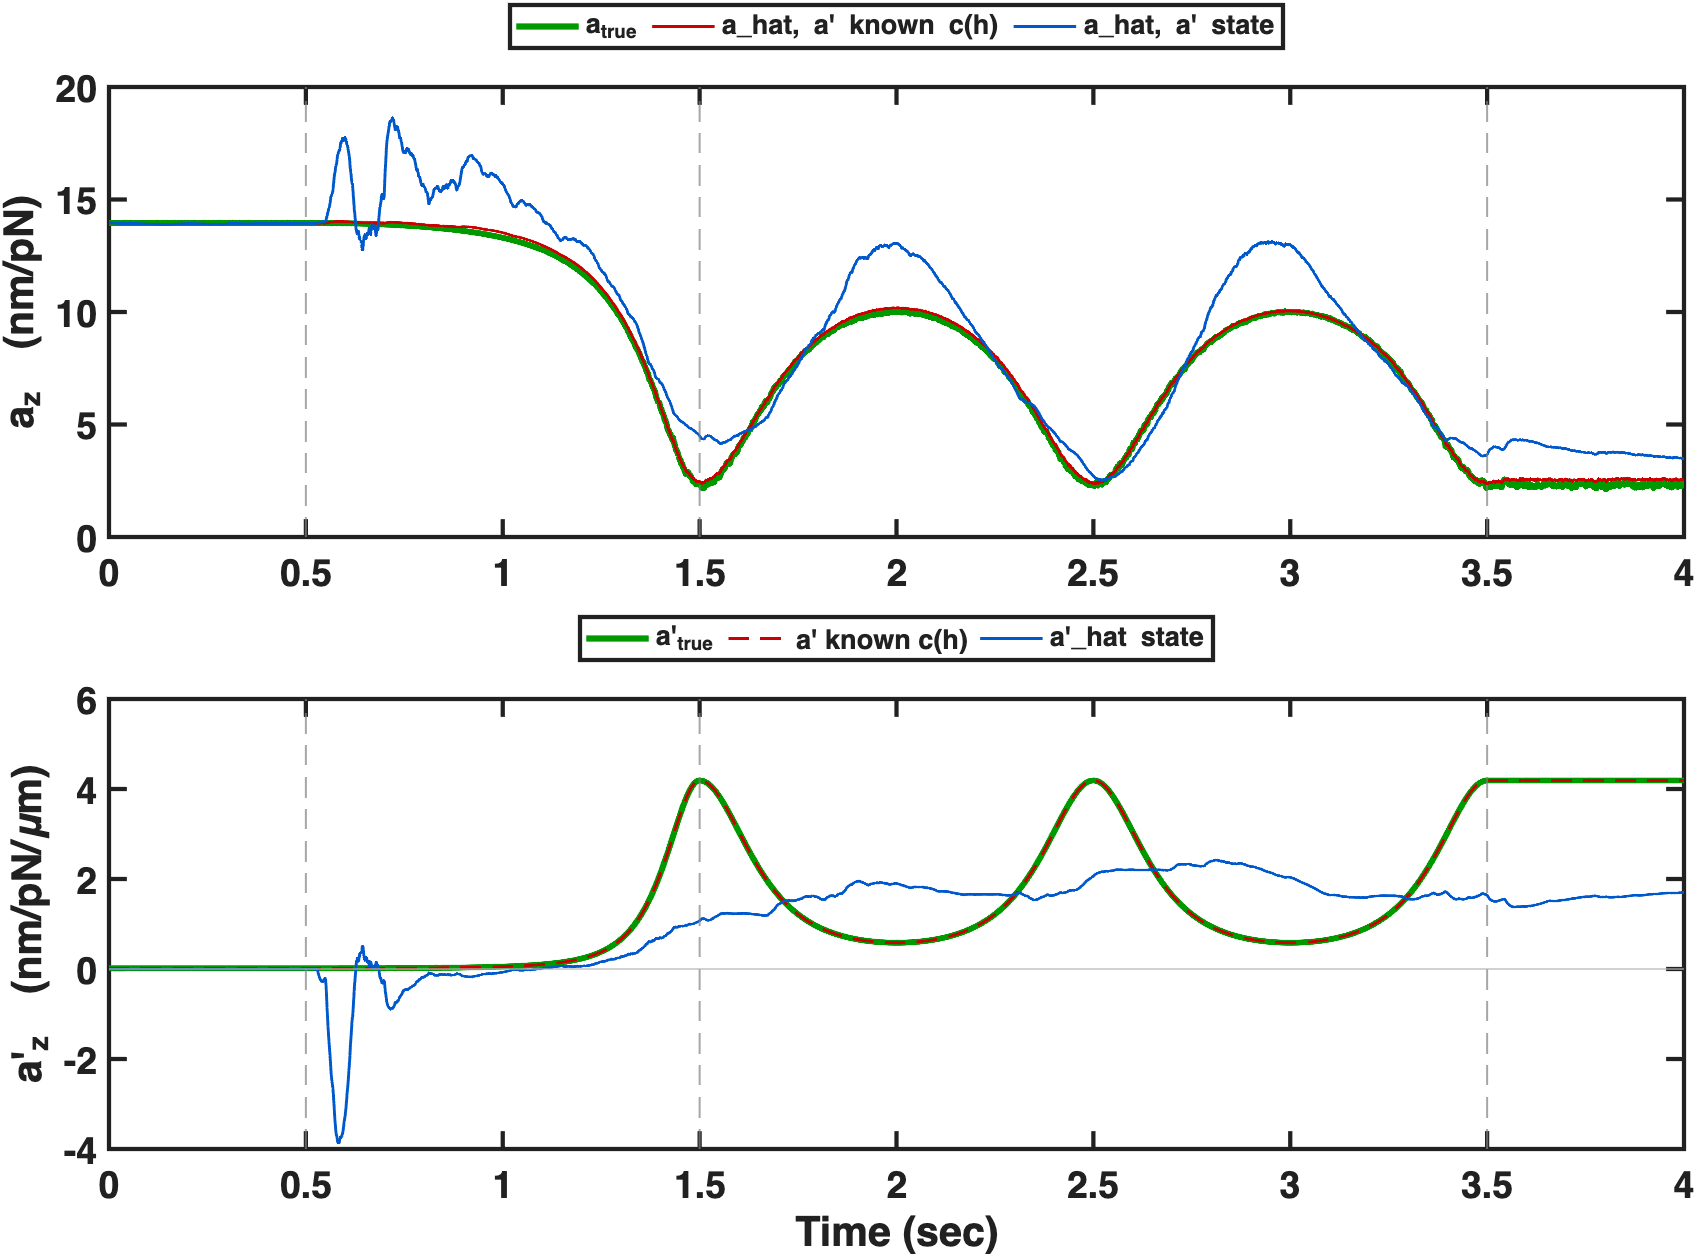
\includegraphics[width=0.88\textwidth]{figures/fig_5state_aprime_overlay_z.png}\\[0.6ex]
{\small\itshape $\hat a_h$ (top) and $a'_{hd}$ (bottom): $a'$ known $c(\bar h)$ vs
$a'$-as-state (both taylor, learning from $t=0$; seed 1, study: 20 seeds).
Study (osc window): known $a'$ $-0.69\%\,/\,3.08\%$ (bias/std); $a'$-as-state
$+6.31\%\,/\,20.7\%$, slope mean $-8.6\%$, trough peaks $\sim\!1/3$ captured,
$P_{55}/\mathrm{Var} = 0.05$. Freeze variant (learn released at $1.5$ s):
$+44.9\%\,/\,74.3\%$, det run diverges --- frozen $a'_{hd}$ also freezes the gain
feedforward.}
\end{minipage}

\end{document}
